\documentclass[12pt]{amsart}
\synctex=1
\setcounter{page}{1}

\hoffset=-.75in
\textwidth=6.5in
\voffset=-.5in
\textheight=9.0in

%\setlength{\textwidth}{4.4in}
%\setlength{\textheight}{7.0in}
%\setlength{\evensidemargin}{1in}
%\setlength{\oddsidemargin}{1in}
%\setlength{\topmargin}{.8in}

\usepackage{ulem}
\usepackage{xcolor}
\usepackage{tikz}

\newtheorem{theorem}{Theorem}%[section]
\newtheorem{lemma}[theorem]{Lemma}

\newtheorem{corollary}[theorem]{Corollary}
\newtheorem{question}[theorem]{Question}

\theoremstyle{definition}
\newtheorem{definition}[theorem]{Definition}
\newtheorem{proposition}[theorem]{Proposition}

\definecolor{mygray}{gray}{0.8}


\begin{document}




\title{Turing Puzzle}


\maketitle

\thispagestyle{empty}




\textbf{Petbotics, Inc.} designs and manufactures (surprise!)
\textbf{robotic pets}.
As per federal law, Petbotics regularly tests their robots to
make sure they won't one day \textbf{rise up and take over the world}.

The testing procedure for one particular model, \textbf{TY-NEE-BAHT},
begins by placing it on the designated space within the blank tape
pictured below.

\begin{center}
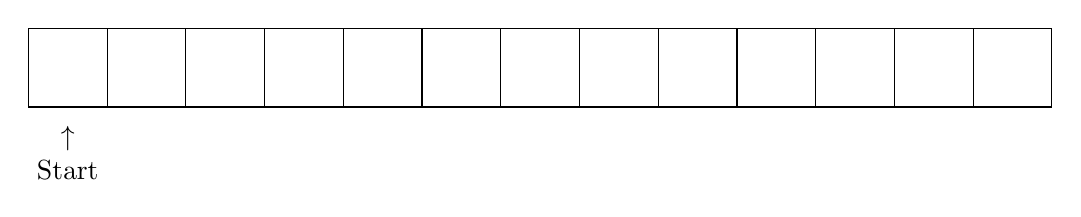
\begin{tikzpicture}
  \draw[step=1] (0,0) grid (13,1);
  \node at (0.5,-0.8) {Start};
  \node at (0.5,-0.4) {\(\uparrow\)};
\end{tikzpicture}
\end{center}

TY-NEE-BAHT uses a combination of its current \textbf{mode} and the
currently drawn \textbf{letter} to decide what to write on the grid and
how to move, based upon the \textbf{TY-NEE-BAHT Program}.
For example:


\newcounter{XPos}

\newcommand{\phCommandColumn}[5]{
\fill[color=lightgray] (\theXPos,3) rectangle +(1,2);
\draw[step=1] (\theXPos,0) grid +(1,5);
\draw[very thick] (\theXPos,3) -- +(1,0);
\node at (\theXPos.5,4.5) {#1};
\node at (\theXPos.5,3.5) {#2};
\node at (\theXPos.5,2.5) {#3};
\node at (\theXPos.5,1.5) {#4};
\node at (\theXPos.5,0.5) {#5};
\stepcounter{XPos}
}

\begin{center}
  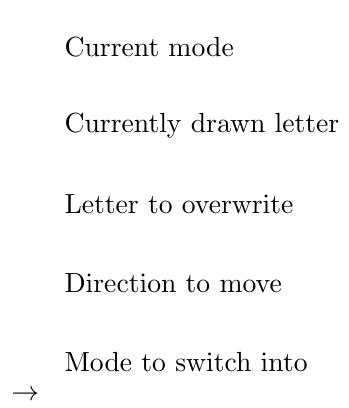
\begin{tikzpicture}

    \phCommandColumn{3}{E}{R}{\(\rightarrow\)}{4}

    \node[anchor=west] at (\theXPos.2,4.5) {Current mode};
    \node[anchor=west] at (\theXPos.2,3.5) {Currently drawn letter};
    \node[anchor=west] at (\theXPos.2,2.5) {Letter to overwrite};
    \node[anchor=west] at (\theXPos.2,1.5) {Direction to move};
    \node[anchor=west] at (\theXPos.2,0.5) {Mode to switch into};
  \end{tikzpicture}
\end{center}

The above instruction directs a TY-NEE-BAHT which is currently
in mode 3 and standing on the letter ``E'' to
\begin{itemize}
\item overwrite the ``E'' with an ``R'',
\item move one square to the right (or loop to the left end of the tape
  if currently on the right end), and
\item switch to mode 4.
\end{itemize}

\textbf{What three-word message will be printed on the blank tape above
when TY-NEE-BAHT powers down?}



TY-NEE-BAHT always begins in mode 1, and
it shuts itself off when it reaches a combination of mode and letter that
is not defined within its program, or after following 1000 instructions.

\begin{center}
  \begin{tikzpicture}[x=0.7cm,y=0.7cm]
    \phCommandColumn{ 1}{ }{A}{\( \rightarrow \)}{10}
    \phCommandColumn{ 1}{G}{ }{\(  \leftarrow \)}{ 8}
    \phCommandColumn{ 1}{J}{V}{\( \rightarrow \)}{ 6}
    \phCommandColumn{ 1}{X}{ }{\( \rightarrow \)}{20}
    \phCommandColumn{ 2}{ }{S}{\(  \leftarrow \)}{11}
    \phCommandColumn{ 2}{A}{A}{\( \rightarrow \)}{14}
    \phCommandColumn{ 2}{E}{F}{\( \rightarrow \)}{ 3}
    \phCommandColumn{ 2}{V}{ }{\( \rightarrow \)}{ 7}
    \phCommandColumn{ 3}{ }{ }{\( \rightarrow \)}{ 2}
    \phCommandColumn{ 3}{E}{R}{\( \rightarrow \)}{ 4}
    \phCommandColumn{ 3}{X}{ }{\(  \leftarrow \)}{17}
    \phCommandColumn{ 3}{Y}{G}{\( \rightarrow \)}{ 1}
    \phCommandColumn{ 4}{ }{ }{\( \rightarrow \)}{ 3}
    \phCommandColumn{ 4}{A}{A}{\(  \leftarrow \)}{13}
    \phCommandColumn{ 4}{J}{G}{\(  \leftarrow \)}{ 1}
    \phCommandColumn{ 4}{E}{E}{\( \rightarrow \)}{ 4}
    \phCommandColumn{ 5}{ }{A}{\( \rightarrow \)}{ 4}
    \phCommandColumn{ 5}{A}{A}{\(  \leftarrow \)}{13}
    \phCommandColumn{ 5}{B}{O}{\(  \leftarrow \)}{19}
    \phCommandColumn{ 5}{J}{Y}{\(  \leftarrow \)}{ 1}
  \end{tikzpicture}
\end{center}
\begin{center}
  \begin{tikzpicture}[x=0.7cm,y=0.7cm]
    \phCommandColumn{ 6}{ }{ }{\( \rightarrow \)}{ 5}
    \phCommandColumn{ 6}{B}{ }{\( \rightarrow \)}{11}
    \phCommandColumn{ 6}{J}{X}{\(  \leftarrow \)}{ 6}
    \phCommandColumn{ 6}{O}{ }{\( \rightarrow \)}{22}
    \phCommandColumn{ 7}{ }{ }{\( \rightarrow \)}{ 6}
    \phCommandColumn{ 7}{G}{J}{\(  \leftarrow \)}{20}
    \phCommandColumn{ 7}{V}{ }{\(  \leftarrow \)}{13}
    \phCommandColumn{ 7}{Y}{B}{\(  \leftarrow \)}{ 6}
    \phCommandColumn{ 8}{ }{ }{\( \rightarrow \)}{ 7}
    \phCommandColumn{ 8}{B}{ }{\( \rightarrow \)}{ 1}
    \phCommandColumn{ 8}{V}{G}{\( \rightarrow \)}{14}
    \phCommandColumn{ 8}{X}{J}{\(  \leftarrow \)}{11}
    \phCommandColumn{ 9}{ }{ }{\( \rightarrow \)}{ 8}
    \phCommandColumn{ 9}{G}{B}{\(  \leftarrow \)}{ 2}
    \phCommandColumn{ 9}{J}{V}{\( \rightarrow \)}{17}
    \phCommandColumn{ 9}{O}{X}{\(  \leftarrow \)}{12}
    \phCommandColumn{10}{ }{ }{\( \rightarrow \)}{ 9}
    \phCommandColumn{10}{B}{G}{\(  \leftarrow \)}{ 3}
    \phCommandColumn{10}{G}{B}{\( \rightarrow \)}{11}
    \phCommandColumn{10}{V}{X}{\( \rightarrow \)}{16}
    \phCommandColumn{11}{ }{ }{\(  \leftarrow \)}{11}
    \phCommandColumn{11}{A}{A}{\(  \leftarrow \)}{12}
    \phCommandColumn{11}{X}{ }{\( \rightarrow \)}{17}
    \phCommandColumn{11}{Y}{ }{\(  \leftarrow \)}{ 4}
  \end{tikzpicture}
\end{center}
\begin{center}
  \begin{tikzpicture}[x=0.7cm,y=0.7cm]
    \phCommandColumn{12}{ }{E}{\(  \leftarrow \)}{12}
    \phCommandColumn{12}{G}{Y}{\(  \leftarrow \)}{ 8}
    \phCommandColumn{12}{A}{A}{\( \rightarrow \)}{ 2}
    \phCommandColumn{12}{Y}{ }{\( \rightarrow \)}{17}
    \phCommandColumn{13}{ }{B}{\( \rightarrow \)}{10}
    \phCommandColumn{13}{E}{M}{\( \rightarrow \)}{ 2}
    \phCommandColumn{13}{J}{ }{\( \rightarrow \)}{ 2}
    \phCommandColumn{13}{S}{S}{\(  \leftarrow \)}{21}
    \phCommandColumn{14}{ }{ }{\( \rightarrow \)}{14}
    \phCommandColumn{14}{V}{ }{\(  \leftarrow \)}{19}
    \phCommandColumn{14}{S}{S}{\( \rightarrow \)}{15}
    \phCommandColumn{14}{Y}{B}{\( \rightarrow \)}{ 4}
    \phCommandColumn{15}{ }{ }{\( \rightarrow \)}{16}
    \phCommandColumn{15}{B}{ }{\( \rightarrow \)}{ 7}
    \phCommandColumn{15}{G}{J}{\(  \leftarrow \)}{13}
    \phCommandColumn{15}{X}{ }{\( \rightarrow \)}{15}
    \phCommandColumn{16}{ }{ }{\( \rightarrow \)}{17}
    \phCommandColumn{16}{G}{B}{\(  \leftarrow \)}{21}
    \phCommandColumn{16}{V}{Y}{\( \rightarrow \)}{ 6}
    \phCommandColumn{16}{O}{J}{\(  \leftarrow \)}{15}
  \end{tikzpicture}
\end{center}

% erasing letters BGJKOXY
\begin{center}
  \begin{tikzpicture}[x=0.7cm,y=0.7cm]
    \phCommandColumn{17}{ }{E}{\(  \leftarrow \)}{18}
    \phCommandColumn{17}{J}{ }{\(  \leftarrow \)}{ 1}
    \phCommandColumn{17}{X}{B}{\( \rightarrow \)}{15}
    \phCommandColumn{17}{Y}{Y}{\(  \leftarrow \)}{ 8}
    \phCommandColumn{18}{ }{ }{\(  \leftarrow \)}{18}
    \phCommandColumn{18}{V}{ }{\(  \leftarrow \)}{12}
    \phCommandColumn{18}{S}{S}{\( \rightarrow \)}{19}
    \phCommandColumn{18}{X}{ }{\(  \leftarrow \)}{ 6}
    \phCommandColumn{19}{ }{A}{\( \rightarrow \)}{20}
    \phCommandColumn{19}{V}{Y}{\(  \leftarrow \)}{ 5}
    \phCommandColumn{19}{X}{B}{\( \rightarrow \)}{14}
    \phCommandColumn{19}{Y}{J}{\( \rightarrow \)}{ 9}
    \phCommandColumn{20}{ }{K}{\(  \leftarrow \)}{ 5}
    \phCommandColumn{20}{G}{B}{\( \rightarrow \)}{12}
    \phCommandColumn{20}{V}{O}{\(  \leftarrow \)}{12}
    \phCommandColumn{20}{Y}{V}{\(  \leftarrow \)}{20}
    \phCommandColumn{21}{ }{S}{\(  \leftarrow \)}{22}
    \phCommandColumn{21}{G}{ }{\(  \leftarrow \)}{ 6}
    \phCommandColumn{21}{J}{B}{\(  \leftarrow \)}{15}
    \phCommandColumn{21}{V}{X}{\( \rightarrow \)}{10}
    \phCommandColumn{22}{ }{N}{\( \rightarrow \)}{ 1}
    \phCommandColumn{22}{B}{G}{\(  \leftarrow \)}{21}
    \phCommandColumn{22}{X}{ }{\( \rightarrow \)}{14}
    \phCommandColumn{22}{Y}{J}{\( \rightarrow \)}{ 7}
  \end{tikzpicture}
\end{center}

\newpage

Solution:

TY-NEE-BAHT's program (essentially a simplified \textbf{Turing machine})
outputs\\ \textbf{AFREEMANSSAKE}, that is, ``A free man's sake'', a reference
to the quest to escape from the control of the machines.







\end{document}
